%
%  wl_hh_benford.tex
%
%  Created by Drew Conway on 2011-02-21
% 
%
\documentclass[xcolor=dvipsnames, 9pt]{beamer}

\newenvironment{code}{\begin{semiverbatim} \begin{footnotesize}}
{\end{footnotesize}\end{semiverbatim}}

% Running Headers and footers
%\usepackage{fancyhdr}

% Multipart figures
%\usepackage{subfigure}

\usepackage{graphicx}
\usepackage{amssymb}
\usepackage{amsfonts}
\usepackage{amsmath}
\usepackage{hyperref}
\usepackage{natbib}
\usepackage{color}
\usepackage{pdfsync}
\usepackage{chancery}
\usepackage{movie15}
\usepackage{pgfpages}
\usepackage{fancyvrb}
\usepackage{colortbl}
\usepackage{wasysym}


% \definecolor{white}{rgb}{255,255,255}
% \definecolor{darkred}{rgb}{0.5,0,0}
% \definecolor{darkgreen}{rgb}{0,0.5,0}
% \definecolor{lightblue}{rgb}{0,0,0.7}

% \hypersetup{colorlinks,
%   linkcolor=white,
%   filecolor=darkred,
%   urlcolor=lightblue,
%   citecolor=darkblue}

\usepackage{beamerthemesplit}
\usetheme{Copenhagen}
\usecolortheme[named=Blue]{structure} 
\setbeamertemplate{navigation symbols}{}
\setbeamertemplate{itemize items}[triangle]
\setbeamertemplate{enumerate items}[default]
%\setbeameroption{show notes on second screen}
%\logo{\includegraphics[width = 2cm]{nyulogo.png}}

\newcommand{\R}{\mathbb{R}}
\renewcommand{\d}{\mathsf{d}}
\newcommand{\dd}{\partial}
\newcommand{\E}{\mathsf{E}}
\newcommand{\bb}{\mathbf}

\title{Citizen Data-Driven Journalism\\The WikiLeaks Afghanistan War Logs}
\author{Drew Conway, Mike Dewar \& John Myles White}
\date{March 9, 2011}

\begin{document}
    
\ifpdf
\DeclareGraphicsExtensions{.pdf, .jpg, .tif}
\else
\DeclareGraphicsExtensions{.eps, .jpg}
\fi
% Set graphics path
\graphicspath{{images/}}

\begin{frame}[plain]
  \titlepage  
\end{frame}



\section{Introduction}

\begin{frame}
	\frametitle{Wikileaks}
	\begin{center}
   % 
\includegraphics[height=0.8\textheight]{wikileaks_eggtimer.png}
    \end{center}
\end{frame}

\begin{frame}
    \frametitle{Data Journalism}
    \begin{center}
    
\includegraphics[width=0.8\textwidth]{guardian.png}
    \end{center}
\end{frame}

\begin{frame}
    \frametitle{Citizen Data Analysis}
    \begin{center}
    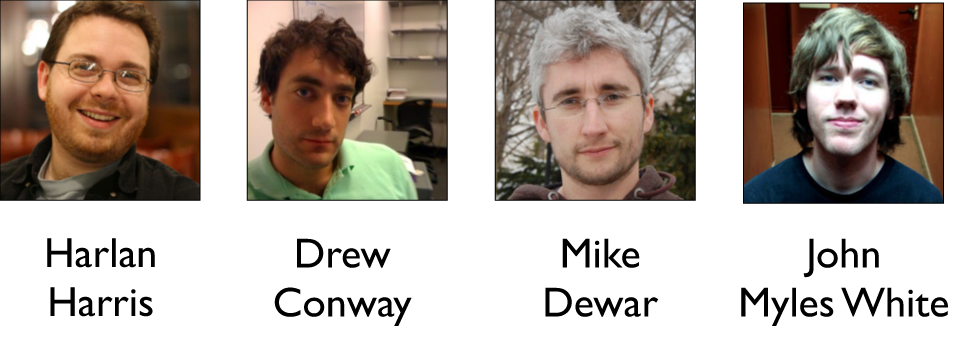
\includegraphics[width=\textwidth]{hackademics.png}
    \end{center}
\end{frame}

{
\setbeamertemplate{background canvas}{
\includegraphics 
	[width=\paperwidth,height=\paperheight]{hackabit.png}} 
\begin{frame}
    \frametitle{Hackabit}
\end{frame}
}

\begin{frame}
    \frametitle{O.S.E.M.N. : A Taxonomy of Data Science}
    
    \begin{center}  
\begin{block}{O.S.E.M.N.}
        \begin{itemize}
            \item \textbf{Obtain} : get the data
            \item \textbf{Scrub} : clean the data
            \item \textbf{Explore} : have a look at the data
            \item \textbf{Model} : try to represent the data
            \item \textbf{iNterpret} : try to understand your model
        \end{itemize}
        \end{block}
        \vspace{2em}
        
\includegraphics[width=0.15\textwidth]{possum.png}
        \hspace{1em}
        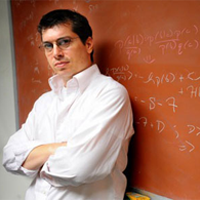
\includegraphics[width=0.15\textwidth]{chris.png}
        \hspace{1em}
        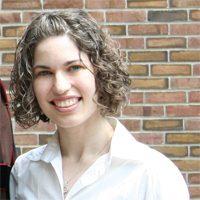
\includegraphics[width=0.15\textwidth]{hilary.png}\\
        Chris Wiggins \& Hilary Mason : \\ \url{http://www.dataists.com/a-taxonomy-of-data-science/}
    \end{center}
\end{frame}

{
\setbeamertemplate{background canvas}{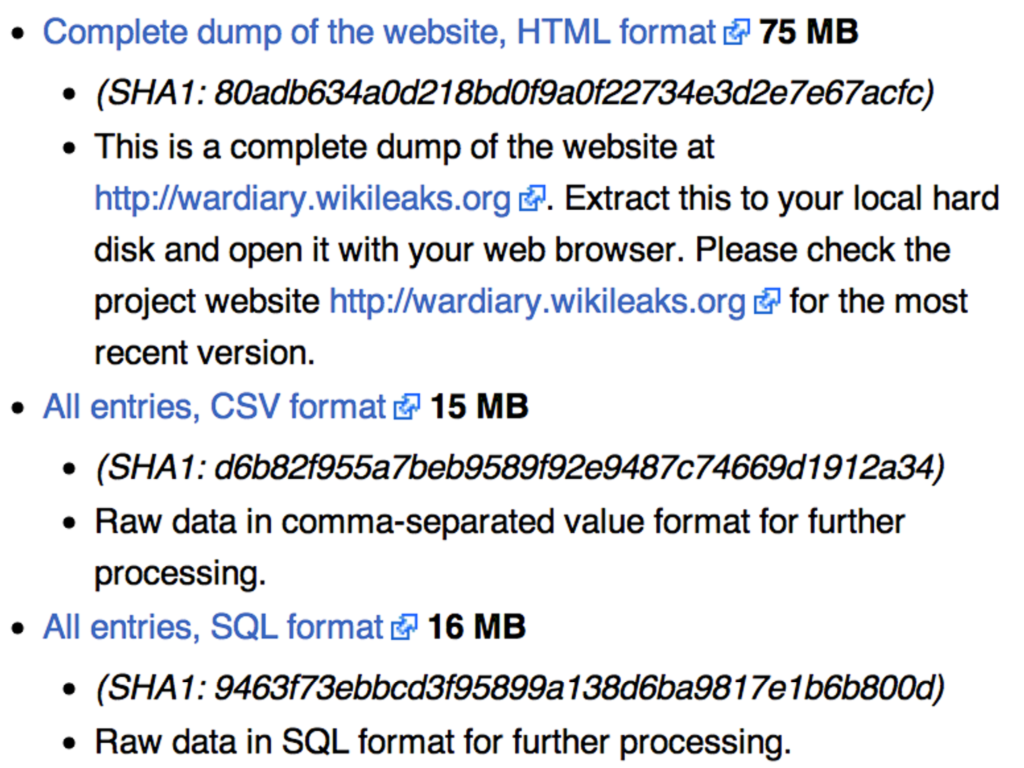
\includegraphics 
	[width=\paperwidth,height=\paperheight]{website.png}} 
\begin{frame}
    \frametitle{Obtain}
\end{frame}
}

\begin{frame}
    \frametitle{Scrub}
    \begin{center}
   % 
\includegraphics[width=0.5\textwidth]{pickaxe.png}
    \end{center}
\end{frame}

{
\setbeamertemplate{background canvas}{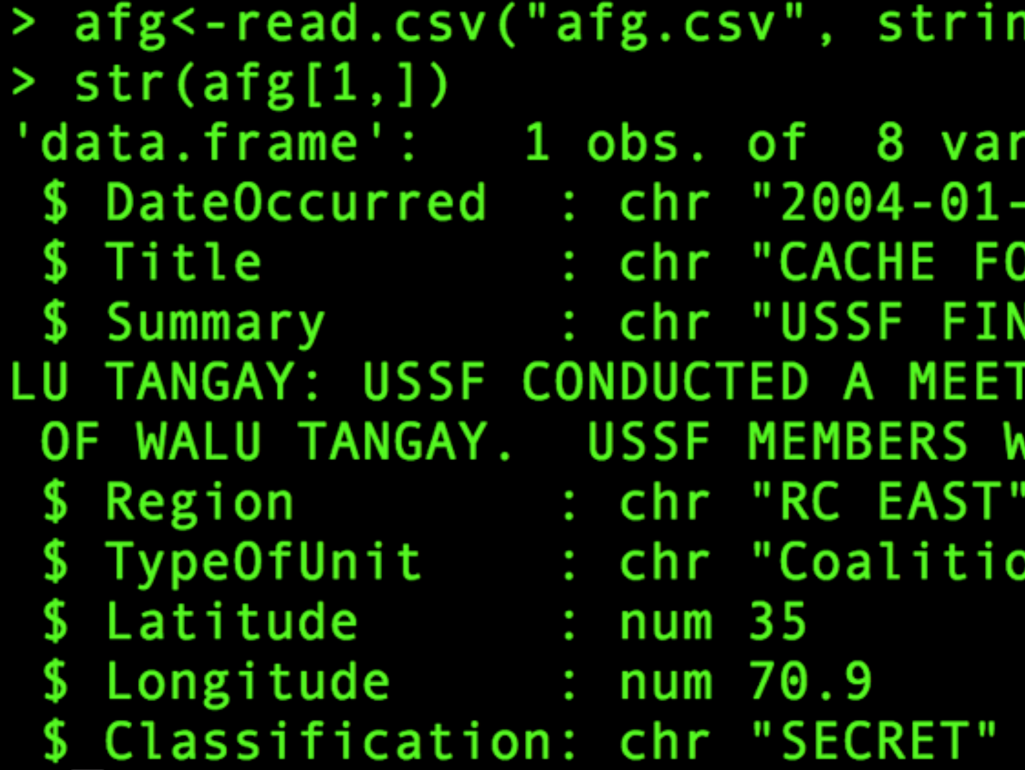
\includegraphics 
	[width=\paperwidth,height=\paperheight]{terminal.png}} 
\begin{frame}
    \frametitle{Explore}
\end{frame}
}

\begin{frame}
    \frametitle{Explore}
    \begin{center}
    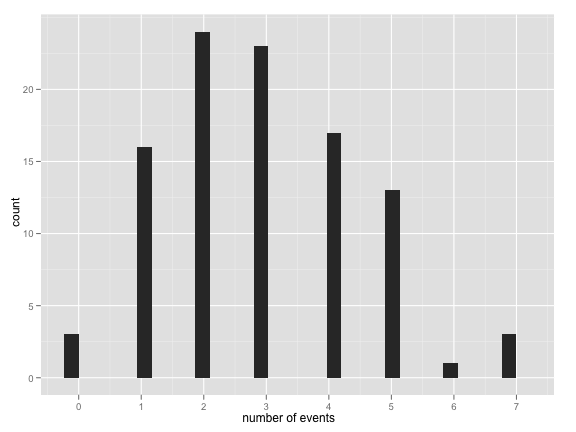
\includegraphics[width=0.9\textwidth]{histogram.png}
    \end{center}
\end{frame}

\begin{frame}
    \frametitle{Model}
    \begin{center}
    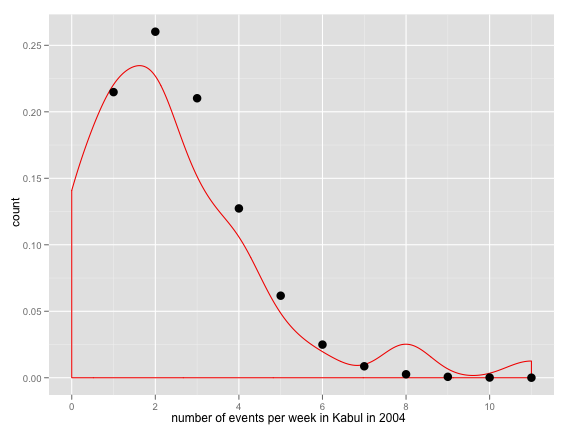
\includegraphics[width=0.9\textwidth]{density_estimate.png}
    \end{center}
\end{frame}

\begin{frame}
    \frametitle{iNterpret}
    \begin{center}
    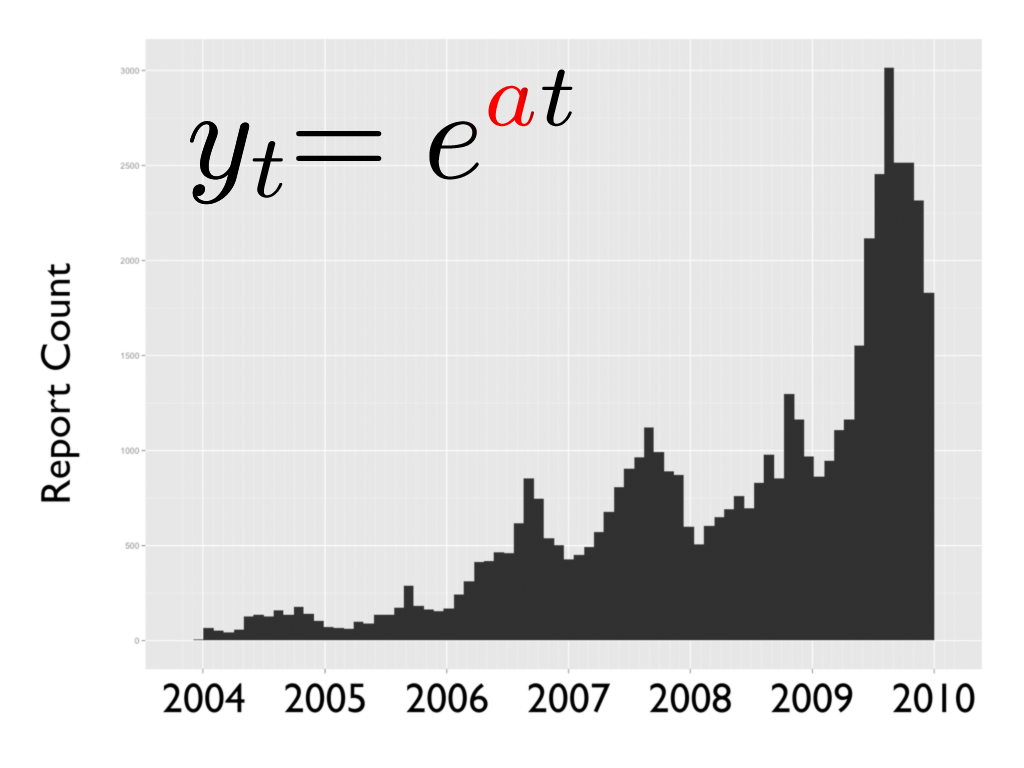
\includegraphics[width=0.9\textwidth]{time_course_model.png}
    \end{center}
\end{frame}

\section{Checking the data} % (fold)
\label{sec:checking_the_data}

\begin{frame}[fragile]
    \frametitle{Why is it important to check the data?}
    \uncover<2->{\begin{center}
        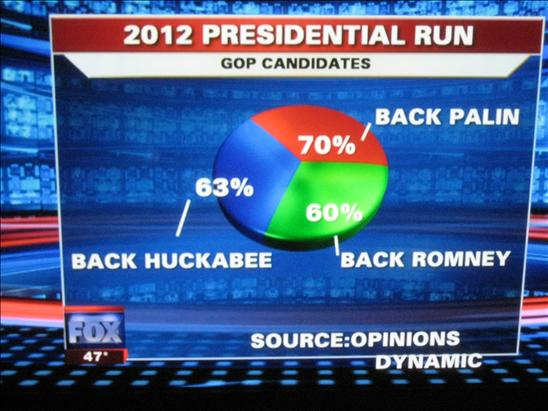
\includegraphics[width=9cm]{fox_news_pie_chart.png}
    \end{center}
    \tiny{\emph{Source}: \href{http://flowingdata.com/2009/11/26/fox-news-makes-the-best-pie-chart-ever/}{http://flowingdata.com/}}}
\end{frame}


\begin{frame}[fragile]
    \frametitle{Greater difficulty in the age of ``big data''}
        With crowd-sourced and dubiously disclosed data we have several issues
        \begin{itemize}
            \item Extremely difficult to vet---especially for non-journalists
            \item Data in ``raw'' form, high degree of variance 
            \item Motivation of sources unknown
        \end{itemize}
        \uncover<2->{\begin{block}{\emph{CJR} -- `The Challenge of Verifying Crowdsourced Information'}
            ``Even though the information from Twitter is not particularly reliable---and things are being retweeted so it’s kind of messy---the basic idea is if you crowdsource the information and put it on one map you can really see the clusters of incidents.  So even though one particular tweet is not that important, if you have similar reports from the media … you can see where the incidents are clustering.''\\
            \hfill{- Jaroslav Valuch, the project manager for Ushahidi Haiti}
        \end{block}}
        \uncover<3->{But...visual evidence can be deceiving
        \begin{itemize}
            \item Need a real test (statistical) to provide better evidence that data is reliable and not fraudulent
        \end{itemize}
        \tiny{Source: `\href{http://www.cjr.org/behind_the_news/the_challenge_of_verifying_cro.php}{The Challenge of Verifying Crowdsourced Information}},' see also: `\href{http://www.cjr.org/campaign_desk/how_wikileaks_outsourced_the_b.php?page=all}{How WikiLeaks Outsourced the Burden of Verification}'}}
\end{frame}

\begin{frame}[fragile]
    \frametitle{How to verify the data}
    First, are we trying to verify the information, or data itself?
    \begin{itemize}
        \item Former requires independent information and resources 
        \item Latter we can do statistically for free! $\smiley$
    \end{itemize}
    \uncover<2->{If simply verifying data as it exists, need a \textbf{data appropriate test}
    \begin{itemize}
        \item What do our data look like?
        \item What is the generating process?
    \end{itemize}}
    \uncover<3->{Journalists often deal with \textbf{discrete count data} wherein additional information has been coded into each event
    \begin{columns}
        \column{.65\textwidth}
            \begin{itemize}
                \item Election:  \# people voting for some candidate per-district
                \item Finance:   \# securities traded per-day
                \item Ushahidi:  \# incidents reported of some type
                \item WikiLeaks: \# SIGACTS per-region or geo-code
            \end{itemize}
        \column{.35\textwidth}
            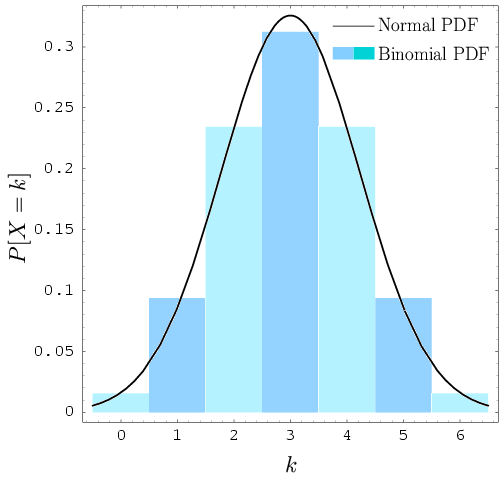
\includegraphics[width=3.2cm]{BinDistApprox_large.png}
    \end{columns}}
    \uncover<4->{We use \textbf{Benford's Law} to test that WikiLeaks data fits a \emph{natural data generating process} for count data}\\
    \uncover<4->{\tiny{Source: \url{http://en.wikipedia.org/wiki/Binomial_distribution}}}
\end{frame}


\begin{frame}[fragile]
    \frametitle{What is Benford's Law}
    \begin{block}{Benford's Law}
       Benford's law, also called the first-digit law, states that in lists of numbers from many (but not all) real-life sources of data, the leading digit is distributed in a specific, non-uniform way. According to this law, the first digit is 1 about 30\% of the time, and larger digits occur as the leading digit with lower and lower frequency, to the point where 9 as a first digit occurs less than 5\% of the time.\\
    \end{block}
    \begin{columns}
        \column{.4\textwidth}
            \uncover<2->{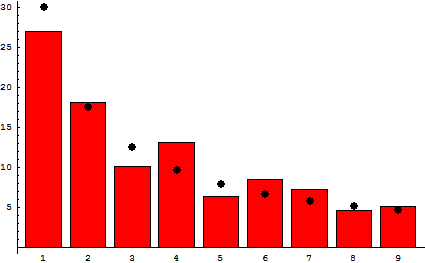
\includegraphics[width=5cm]{Benfords_law_illustrated_by_world's_countries_population.png}}\\
        \column{.6\textwidth}
            \begin{itemize}
                \uncover<2->{\item Distribution of first digits in the population of the 237 countries of the world (at left)}
                \uncover<3->{\item Detect check fraud (\href{http://www.journalofaccountancy.com/Issues/1999/May/nigrini}{\emph{Journal of Accountancy}})
                
                \item Election rigging in Iran (\href{http://www.fivethirtyeight.com/2009/06/statistical-evidence-does-not-prove.html}{FiveThirtyEight})}
            \end{itemize}
    \end{columns}
    \vspace{2mm}
    \uncover<4->{For the WikiLeaks, we will analyze the leading digits for \textbf{weekly counts of SIGACT reports} in the data
    \begin{itemize}
        \item This includes visual and statistical tests with Benford's Law
    \end{itemize}}
    \uncover<4->{\tiny{Source: \url{http://en.wikipedia.org/wiki/Benford's_law}}}
\end{frame}

%\begin{frame}[fragile]
%    \frametitle{Running the test}
%    \begin{columns}
%        \column{.8\textwidth}
%            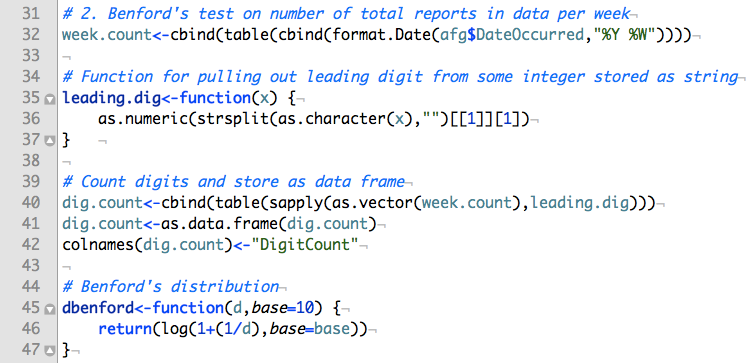
\includegraphics[width=9.2cm]{r_code1.png}
%        \column{.2\textwidth}
%            \only<2>{\alert{\textbf{\Huge{$\leftarrow$}}}} \\
%            \vspace{8mm}
%            \only<3>{\alert{\textbf{\Huge{$\leftarrow$}}}} % yo I can't compile if this \\ is left here!
%            \vspace{1.5cm}
%            \only<4>{\alert{\textbf{\Huge{$\leftarrow$}}}}
%            \vspace{1.7cm}
%    \end{columns}
%    \vspace{1mm}
%    \hline
%    \begin{columns}
%        \column{.33\textwidth}
%            \begin{center}
%                \uncover<2->{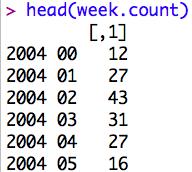
\includegraphics[width=2cm]{r_code2.png}}
%            \end{center}
%        \column{.33\textwidth}
%            \begin{center}
%                \uncover<2->{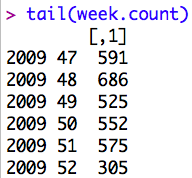
\includegraphics[width=2cm]{r_code2_5.png}}
%            \end{center}
%        \column{.33\textwidth}
%            \begin{center}
%                \uncover<4->{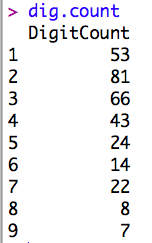
\includegraphics[width=1.7cm]{r_code3.png}}
%            \end{center}
%    \end{columns}
%\end{frame} 

\begin{frame}[fragile]
    \frametitle{Results 1 -- all of the data}
        \begin{columns}
            \column{.7\textwidth}
                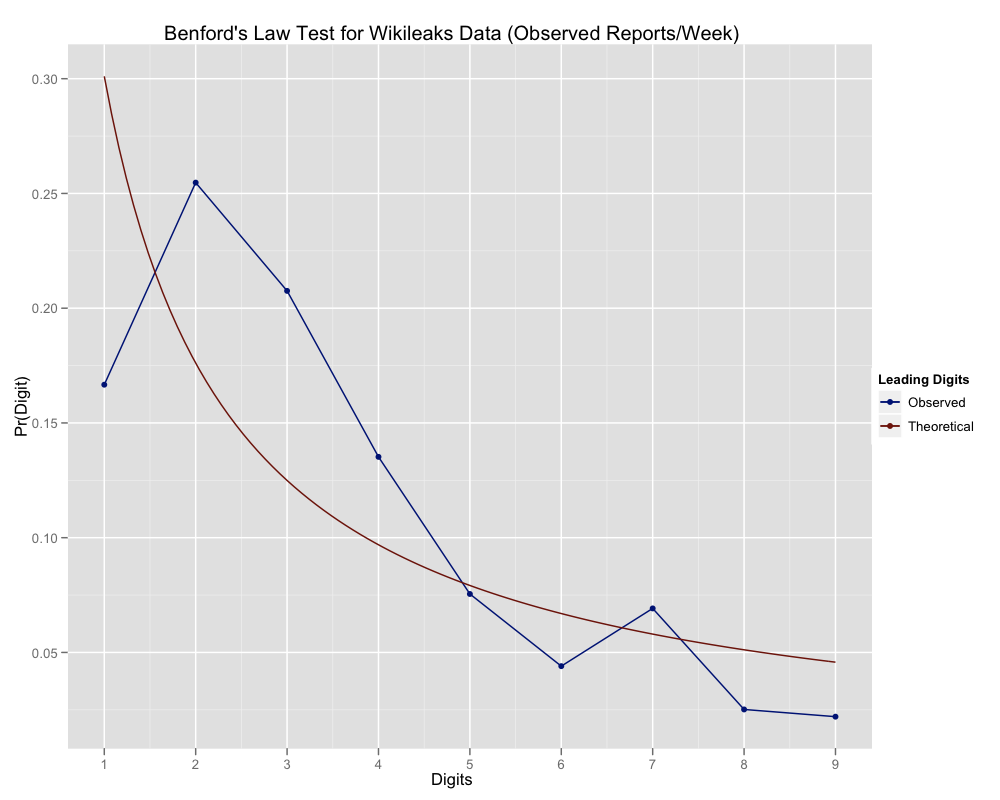
\includegraphics[width=8.5cm]{benford_all.png}
            \column{.3\textwidth}
            Chi-squared goodness of fit test
            \begin{itemize}
                \item $\chi^{2}=72$
                \item p-value=0.23
            \end{itemize}
            \vspace{3.3cm}
        \end{columns}
        \textbf{Cannot reject null} that data came from Benford-like data generating process}
\end{frame}

\begin{frame}[fragile]
    \frametitle{Results 2 -- by region}
    \begin{center}
        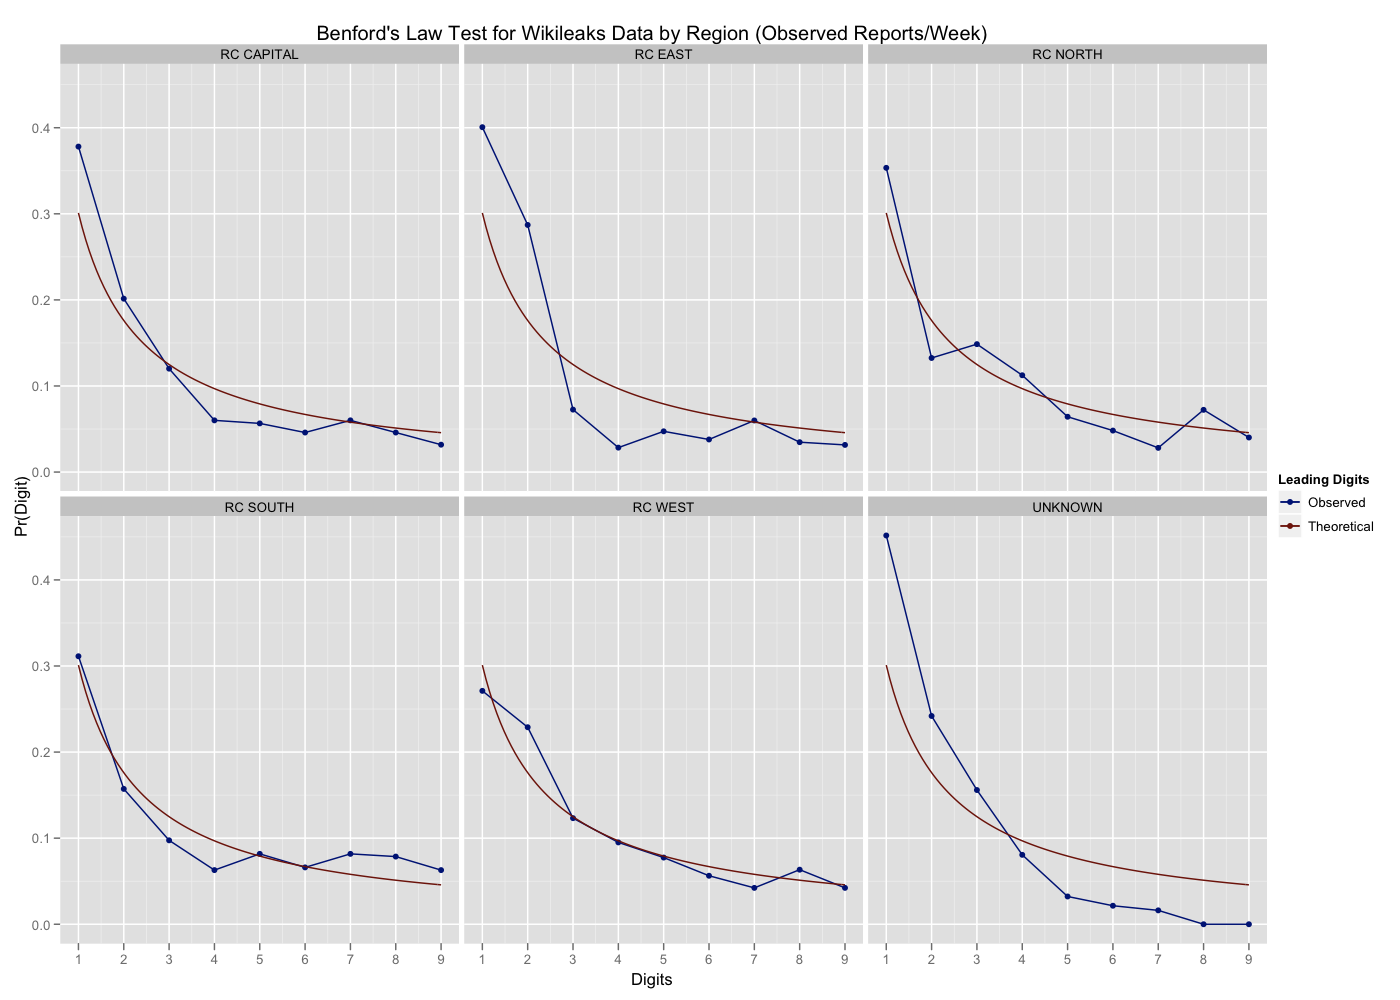
\includegraphics[width=10cm]{benford_region.png}
    \end{center}
\end{frame}

% section checking_the_data (end)

\section{Other analyses} % (fold)
\label{sec:other_analyses}

\begin{frame}[fragile]
  \frametitle{Seasonality}
  \begin{center}
    % 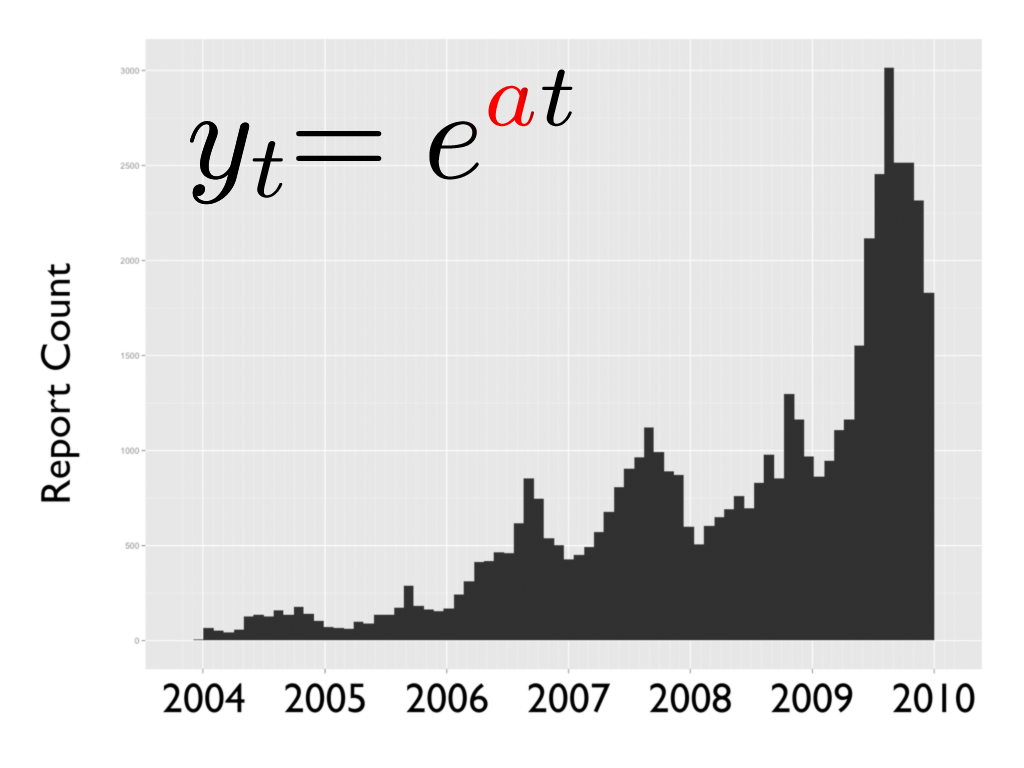
\includegraphics[width = 8.5cm]{time_course.png}
  \end{center}
\end{frame}

\begin{frame}[fragile]
  \frametitle{Seasonal Trend}
  \begin{itemize}
    \item{We see a clear seasonal trend with peaks of activity repeating midway through each year}
    \item{Why is this reasonable to expect?}
  \end{itemize}
\end{frame}

\begin{frame}[fragile]
  \frametitle{Summer Violence across the World}
  \begin{itemize}
    \item{Well-known studies show increased violence during the summer across the world}
    \item{In Afghanistan, summer is officially declared as the fighting season}
    \item{In Britain, injuries and deaths from violence peak during the summer}
    \item{In Norway, the length of day correlates with increased violence}
    \item{In Africa, there are (disputed) claims that hotter climates are associated with greater incidence of war}
  \end{itemize}
\end{frame}

\begin{frame}[fragile]
  \frametitle{Afghanistan's Climate}
  \begin{itemize}
    \item{Afghanistan is a mountainous country with harsh winters}
    \item{Winter Temperatures: $\sim$ -10 F}
    \item{Summer Temperatures: $\sim$ 122 F}
  \end{itemize}
\end{frame}

%http://www.independent.co.uk/news/uk/this-britain/violence-prone-to-seasonal-variations-693678.html
%http://www.rockefellerfoundation.org/uploads/files/526ba3ae-0123-4b9e-b955-f952be8a40bc-warming.pdf
%http://www.ncbi.nlm.nih.gov/pubmed/11007723
%http://www.nytimes.com/2010/01/12/world/asia/12afghan.html

%\begin{frame}[fragile]
%  \frametitle{Cautious Interpretation}
%  \begin{itemize}
%    \item{But we should be cautious about interpreting this relationship as a causal process}
%    \item{In the U.S., ice cream sales go up during the summer, the same time of year when the crime rate goes up}
%    \item{But we don't think that ice cream causes crime}
%    \item{Observing a pattern is not the same thing as understanding its origins}
%  \end{itemize}
%\end{frame}

\begin{frame}[fragile]
  \frametitle{Text Analysis}
  
  \begin{itemize}
    \item{Every event in the Wikileaks data set has an ad hoc text summary}
    \item{We conducted two types of text analysis:}
    \begin{enumerate}
      \item{Grouping similar types of events using LDA}
      \item{Identifying what makes Wikileaks text different from normal English text using outlier words}
    \end{enumerate}
  \end{itemize}
\end{frame}

\begin{frame}[fragile]
  \frametitle{LDA}
  \begin{itemize}
    \item{LDA stands for Latent Dirichlet Allocation}
    \item{LDA provides a fully automatic method for clustering documents into categories}
    \item{Categories are called topics and are characterized by a set of words that distinguish that topic from other topics}
  \end{itemize}
\end{frame}

\begin{frame}[fragile]
  \frametitle{LDA Example}
  \begin{itemize}
    \item{The classic example of LDA in action is the categorization of scientific articles}
    \item{Blei et al. analyzed the corpus of Science magazine between 1880 and 2002}
    \item{LDA extracted interpretable topics matching subfields of science}
  \end{itemize}
\end{frame}

\begin{frame}[fragile]
  \frametitle{Four Topics from the Science Corpus}
  
  \begin{center}
    \begin{tabular}{cccc}
      human & evolution & disease & computer \\
      genome & evolutionary & host & models \\
      dna & species & bacteria & information \\
      genetic & organisms & diseases & data \\
      genes & life & resistance & computers \\
      sequence & origin & bacterial & system \\
      gene & biology & new & network \\
      molecular & groups & strains & systems \\
      sequencing & phylogenetic & control & model \\
      map & living & infectious & parallel \\
      information & diversity & malaria & methods \\
      genetics & group & parasite & networks \\
      mapping & new & parasites & software \\
      project & two & united & new \\
      sequences & common & tuberculosis & simulations \\
    \end{tabular}
  \end{center}
\end{frame}

\begin{frame}[fragile]
  \frametitle{LDA Details}
  
  \begin{itemize}
    \item{For more (technical) details, see 
\href{http://www.cs.princeton.edu/$\sim$blei/modeling-science.pdf}{http://www.cs.princeton.edu/$\sim$blei/modeling-science.pdf}}
    \item{Many R packages implement LDA, including ``LDA'' and ``topicmodels''}
  \end{itemize}
\end{frame}

\begin{frame}[fragile]
  \frametitle{LDA and the Wikileaks Data}
  
  \begin{itemize}
    \item{Use the summary text for each event}
    \item{Assume that there are 10 topics}
    \item{Estimate topics for each region and each year separately}
    \item{Make plots}
  \end{itemize}
\end{frame}

\begin{frame}[fragile]
  TOPIC PLOT GOES HERE
\end{frame}

\begin{frame}
  \frametitle{Outlier Words}
  
  \begin{itemize}
    \item{LDA groups the events in the Wikileaks data based on their summaries}
    \item{But what makes the Wikileaks data different from other text?}
  \end{itemize}
\end{frame}

\begin{frame}[fragile]
  \frametitle{Outlier Analysis}
  
  \begin{itemize}
    \item{Take a standard English corpus: here, we'll use Wikipedia.}
    \item{Compare frequency of words in Wikileaks data against frequency of words in normal English}
    \item{From words that are unusually frequent in Wikileaks text, select most interesting few}
    \item{Visualize}
  \end{itemize}
\end{frame}

\begin{frame}
  OUTLIER WORDS PLOTS GO HERE
\end{frame}

\begin{frame}[fragile]
  \frametitle{What's Left to Do?}
  
  \begin{itemize}
    \item{Generated lots of maps of Afghanistan showing topics, special words, etc., etc.}
    \item{But would like something that combines the spatial information of a map with the temporal information we saw in earlier plots}
    \item{How? Build an animation}
  \end{itemize}
\end{frame}

\begin{frame}[fragile]
  \frametitle{Building an Animation}
  
  \begin{itemize}
    \item{Use a mathematical model to smooth data within 3 month bins, shift bin forward day by day}
    \item{Generate image for every bin}
    \item{Use ffmpeg to compile images into an animation}
  \end{itemize}
\end{frame}

% SHOW ANIMATION AS SEPARATE VIDEO

% section other_analyses (end)

\end{document}
